\documentclass{article}

\usepackage{KjelsethReportStyle}

%   ############################## Customisation ##############################

% Document metadata
\title{\fontsize{24}{36}\selectfont Programable Logic Circuts\\ %Edit title here \\ means new line
Lab 06} % Line 2 of title, its not subtitle, that is possible to, google it
\author{{\ttfamily Sølve Kjelseth}} % Input your name, replace \ttfamily with \normalfont to make it not monospaced but regular font (removing \ttfamily will not do this because of the monospaced font inside tables command, and author is technically a 1x1 table)
\date{\today} % Auto updates the date, untill you export it, replace with hardcoded date if you need

%   ############################## Document begins here ##############################
\begin{document}

\maketitle % Makes title front page based on the title, author and date metadata, change at the top



%   ############################## Section ##############################
\addtocontents{toc}{\protect\setcounter{tocdepth}{0}} % Temporarily hide from TOC
\section{Introduction} % Numbered section named Introduction
This is the sixth report in this course, detailing the completion of the sixth lab exercise. With the purpose is to investigate Finite State Machines (FSM).\par
Note: As always, the \LaTeX\ code is open source, see
\linkgithub{my GitHub {
\begingroup
\setbox0=\hbox{
\includegraphics[scale=0.5]{Figures/github-mark.png}}%
\parbox{\wd0}{\box0}
\endgroup}}

\clearpage
\tableofcontents % Generate TOC
\hfill
\listoffigures % List of figures
\hfill
\listoftables % List of tables
\addtocontents{toc}{\protect\setcounter{tocdepth}{2}} % Restore TOC depth



%   ############################## Section ##############################
\section{Part 1}
This Part is about making a FSM using structural assignments, it is kind of divided into two parts with different types of one-hot encoding, one where the reset state, \(A\), is \verb|000000001|, and one where \(A\) is \verb|000000000| but for any other state the last bit is \verb|1| in addition to the encoding one-hot bit.

\subsection{Solving}
Solving this task was done by making table~\ref{tab:states} and finding a boolean expression for each bit. Then the output was connected directly to the encoding to display it on the first 9 LED's. The final 10th LED was connected to the states that signifies on output of the system. For the the part with the different one-hot encoding only a few adjustments was needed.


% Table generated by Excel2LaTeX from sheet 'Part 1 OldEncoding'
\begin{table}[htbp]
  \centering
  \tabcaption{State change table}
    \resizebox{\textwidth}{!}{%
    \begin{tabular}{|c|c|c|c|c|c|c|c|c|c|c|c|c|c|c|c|c|c|c|c|c|}
    \hline
    \multicolumn{10}{|c|}{Current state}                                          & Input & \multicolumn{10}{c|}{New state} \bigstrut\\
    \hline
    Name  & Y8    & Y7    & Y6    & Y5    & Y4    & Y3    & Y2    & Y1    & Y0    & w     & Name  & Y8'   & Y7'   & Y6'   & Y5'   & Y4'   & Y3'   & Y2'   & Y1'   & Y0' \bigstrut\\
    \hline
    A     & 0     & 0     & 0     & 0     & 0     & 0     & 0     & 0     & 1     & 0     & B     & 0     & 0     & 0     & 0     & 0     & 0     & 0     & 1     & 0 \bigstrut\\
    \hline
    A     & 0     & 0     & 0     & 0     & 0     & 0     & 0     & 0     & 1     & 1     & F     & 0     & 0     & 0     & 1     & 0     & 0     & 0     & 0     & 0 \bigstrut\\
    \hline
    B     & 0     & 0     & 0     & 0     & 0     & 0     & 0     & 1     & 0     & 0     & C     & 0     & 0     & 0     & 0     & 0     & 0     & 1     & 0     & 0 \bigstrut\\
    \hline
    B     & 0     & 0     & 0     & 0     & 0     & 0     & 0     & 1     & 0     & 1     & F     & 0     & 0     & 0     & 1     & 0     & 0     & 0     & 0     & 0 \bigstrut\\
    \hline
    C     & 0     & 0     & 0     & 0     & 0     & 0     & 1     & 0     & 0     & 0     & D     & 0     & 0     & 0     & 0     & 0     & 1     & 0     & 0     & 0 \bigstrut\\
    \hline
    C     & 0     & 0     & 0     & 0     & 0     & 0     & 1     & 0     & 0     & 1     & F     & 0     & 0     & 0     & 1     & 0     & 0     & 0     & 0     & 0 \bigstrut\\
    \hline
    D     & 0     & 0     & 0     & 0     & 0     & 1     & 0     & 0     & 0     & 0     & E     & 0     & 0     & 0     & 0     & 1     & 0     & 0     & 0     & 0 \bigstrut\\
    \hline
    D     & 0     & 0     & 0     & 0     & 0     & 1     & 0     & 0     & 0     & 1     & F     & 0     & 0     & 0     & 1     & 0     & 0     & 0     & 0     & 0 \bigstrut\\
    \hline
    E     & 0     & 0     & 0     & 0     & 1     & 0     & 0     & 0     & 0     & 0     & E     & 0     & 0     & 0     & 0     & 1     & 0     & 0     & 0     & 0 \bigstrut\\
    \hline
    E     & 0     & 0     & 0     & 0     & 1     & 0     & 0     & 0     & 0     & 1     & F     & 0     & 0     & 0     & 1     & 0     & 0     & 0     & 0     & 0 \bigstrut\\
    \hline
    F     & 0     & 0     & 0     & 1     & 0     & 0     & 0     & 0     & 0     & 0     & B     & 0     & 0     & 0     & 0     & 0     & 0     & 0     & 1     & 0 \bigstrut\\
    \hline
    F     & 0     & 0     & 0     & 1     & 0     & 0     & 0     & 0     & 0     & 1     & G     & 0     & 0     & 1     & 0     & 0     & 0     & 0     & 0     & 0 \bigstrut\\
    \hline
    G     & 0     & 0     & 1     & 0     & 0     & 0     & 0     & 0     & 0     & 0     & B     & 0     & 0     & 0     & 0     & 0     & 0     & 0     & 1     & 0 \bigstrut\\
    \hline
    G     & 0     & 0     & 1     & 0     & 0     & 0     & 0     & 0     & 0     & 1     & H     & 0     & 1     & 0     & 0     & 0     & 0     & 0     & 0     & 0 \bigstrut\\
    \hline
    H     & 0     & 1     & 0     & 0     & 0     & 0     & 0     & 0     & 0     & 0     & B     & 0     & 0     & 0     & 0     & 0     & 0     & 0     & 1     & 0 \bigstrut\\
    \hline
    H     & 0     & 1     & 0     & 0     & 0     & 0     & 0     & 0     & 0     & 1     & I     & 1     & 0     & 0     & 0     & 0     & 0     & 0     & 0     & 0 \bigstrut\\
    \hline
    I     & 1     & 0     & 0     & 0     & 0     & 0     & 0     & 0     & 0     & 0     & B     & 0     & 0     & 0     & 0     & 0     & 0     & 0     & 1     & 0 \bigstrut\\
    \hline
    I     & 1     & 0     & 0     & 0     & 0     & 0     & 0     & 0     & 0     & 1     & I     & 1     & 0     & 0     & 0     & 0     & 0     & 0     & 0     & 0 \bigstrut\\
    \hline
    \end{tabular}}%
  \label{tab:states}%
\end{table}%



\clearpage
\subsection{Code}
\writecode[VHDL]{Part1_TLE_old.vhd}{TLE with the first type of one-hot}
\clearpage
\writecode[VHDL]{Part1_states_old.vhd}{State register first type}
The only thing changed for the second type is a few assignments in the TLE and the register uses a true zero reset instead of the last bit as \verb|1|.

\clearpage
\writecode[VHDL]{Part1_TLE_new.vhd}{TLE with the second type of one-hot}
\clearpage
\writecode[VHDL]{Part1_states_new.vhd}{State register second type}

\clearpage
\subsection{RTL}

\begin{figure}[h]
    \centering
    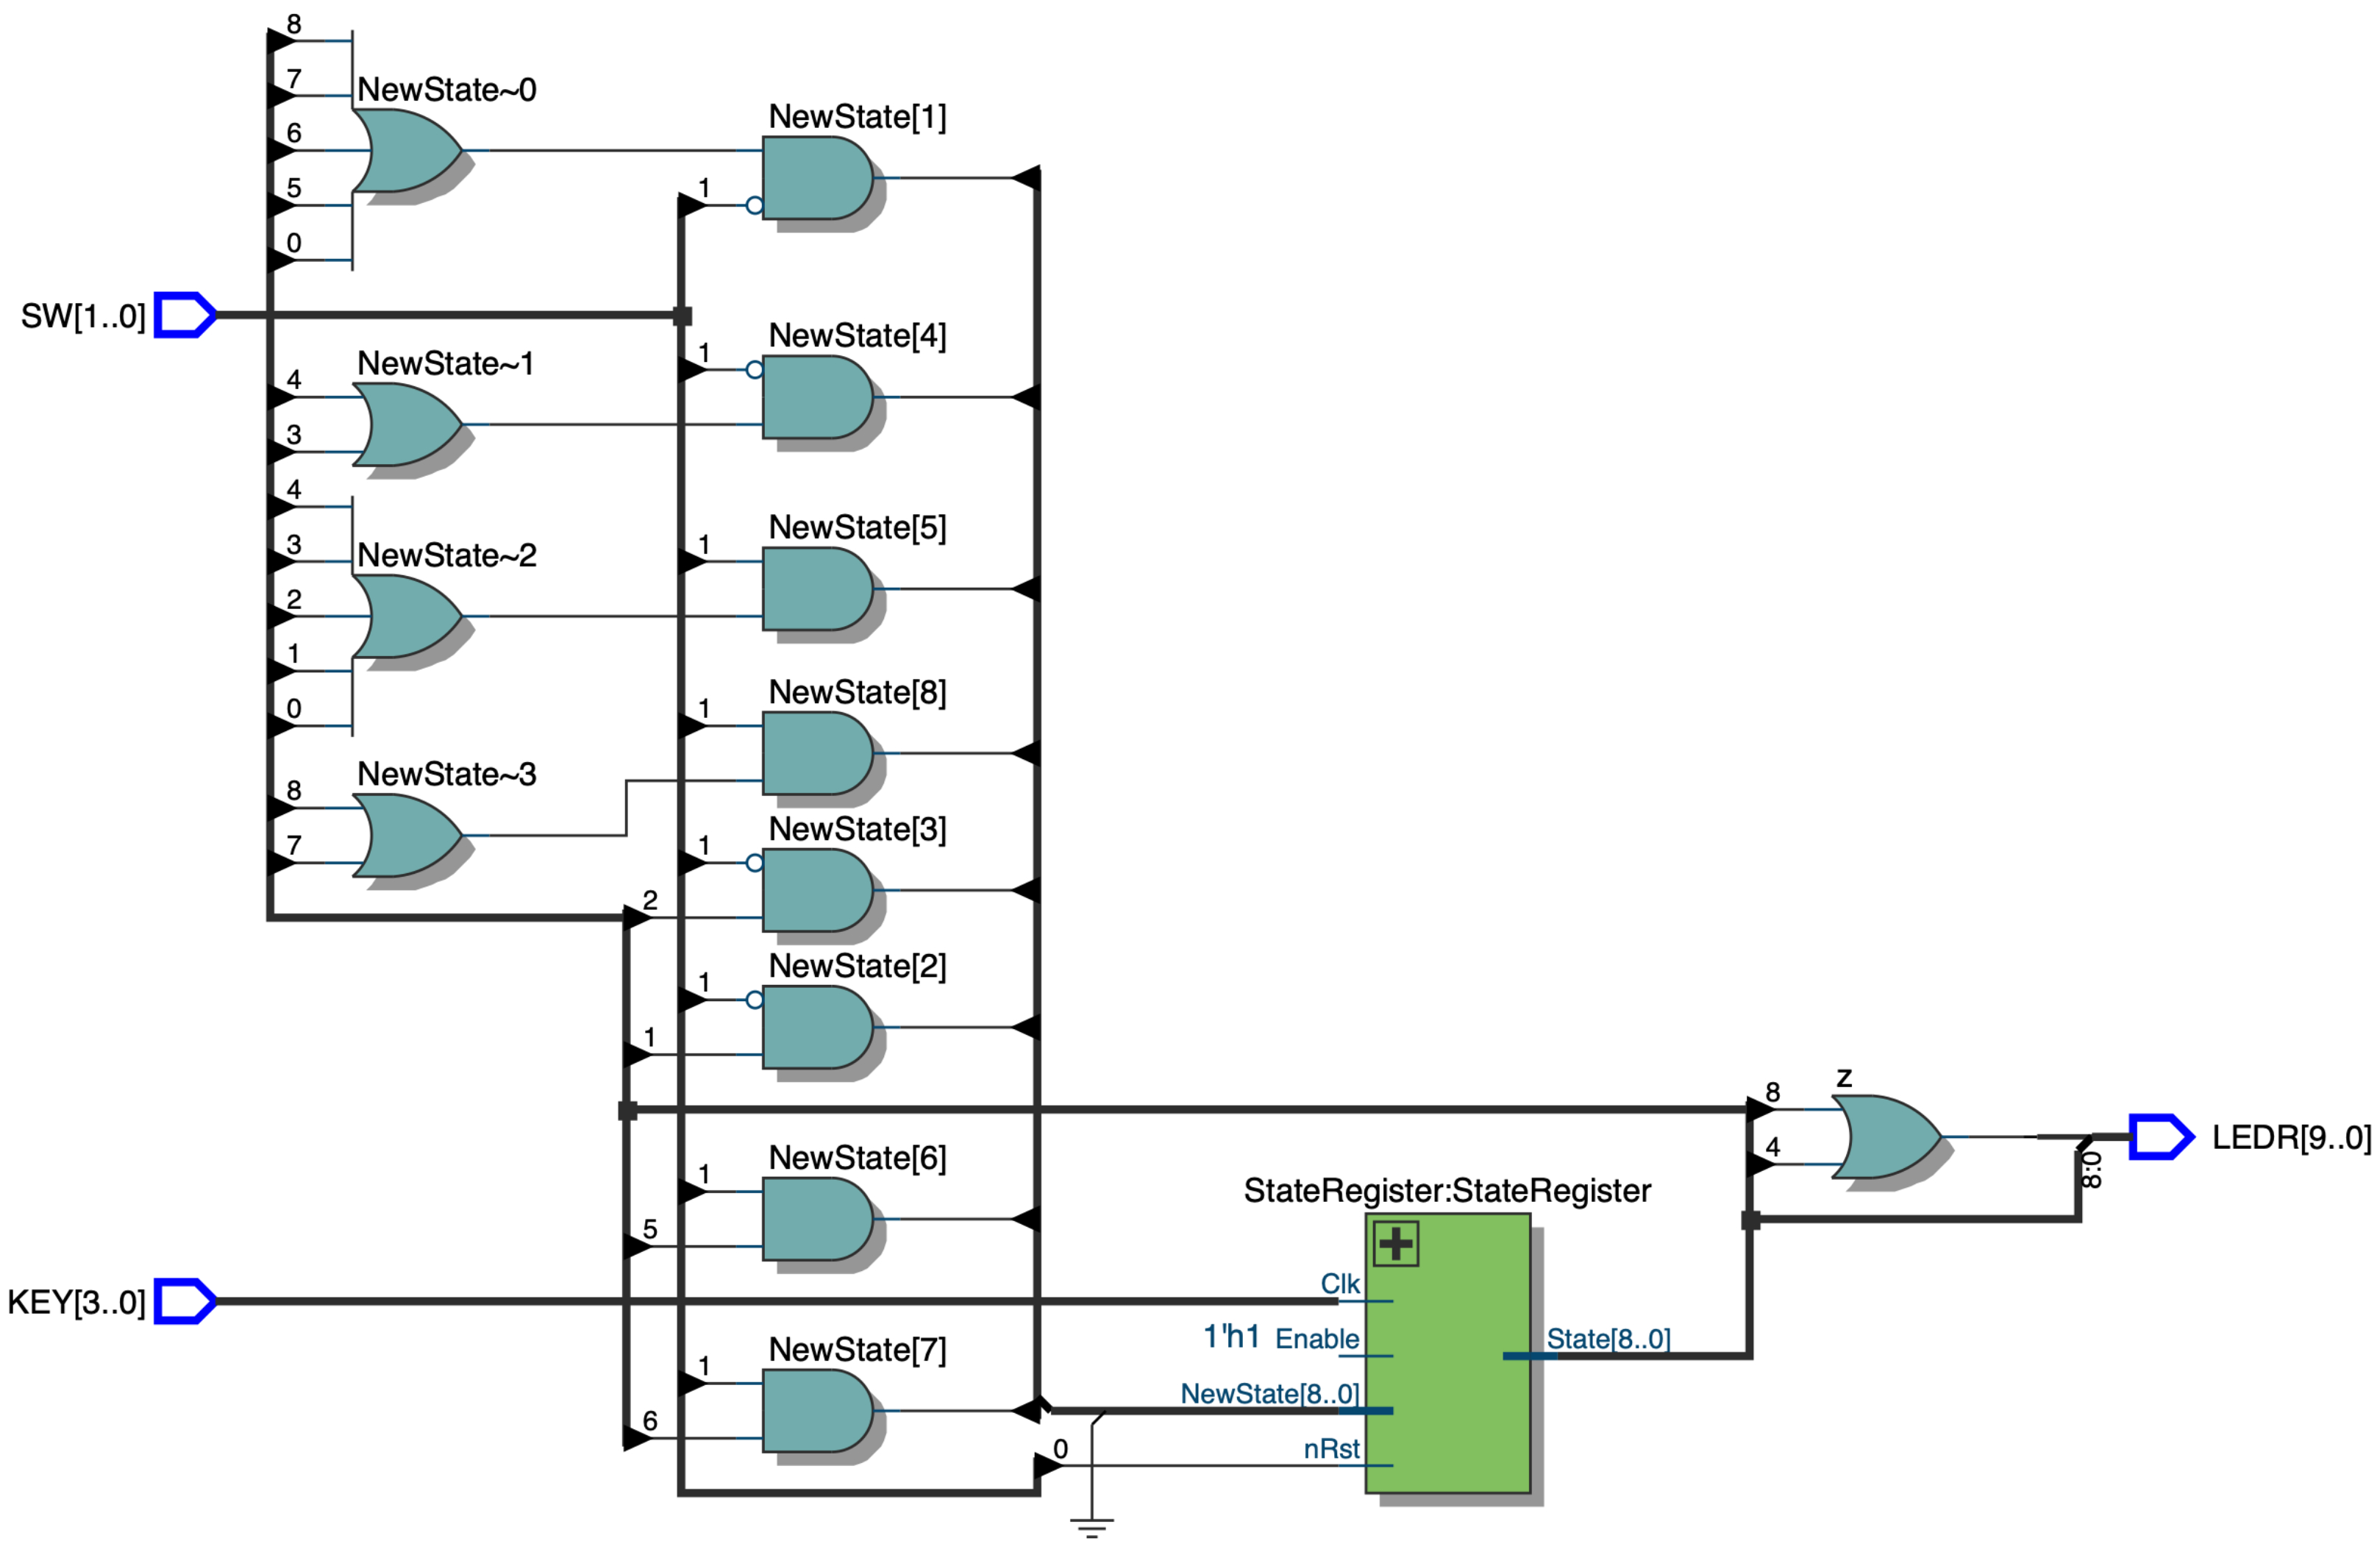
\includegraphics[width=1\textwidth]{Figures/Part1_RTL_TLE_old.jpg}
    \figcaption{RTL of the TLE with the first type one-hot encoding}
    \label{fig:p1_RTL_TLE_old}
\end{figure}
\hfill
\begin{figure}[h]
    \centering
    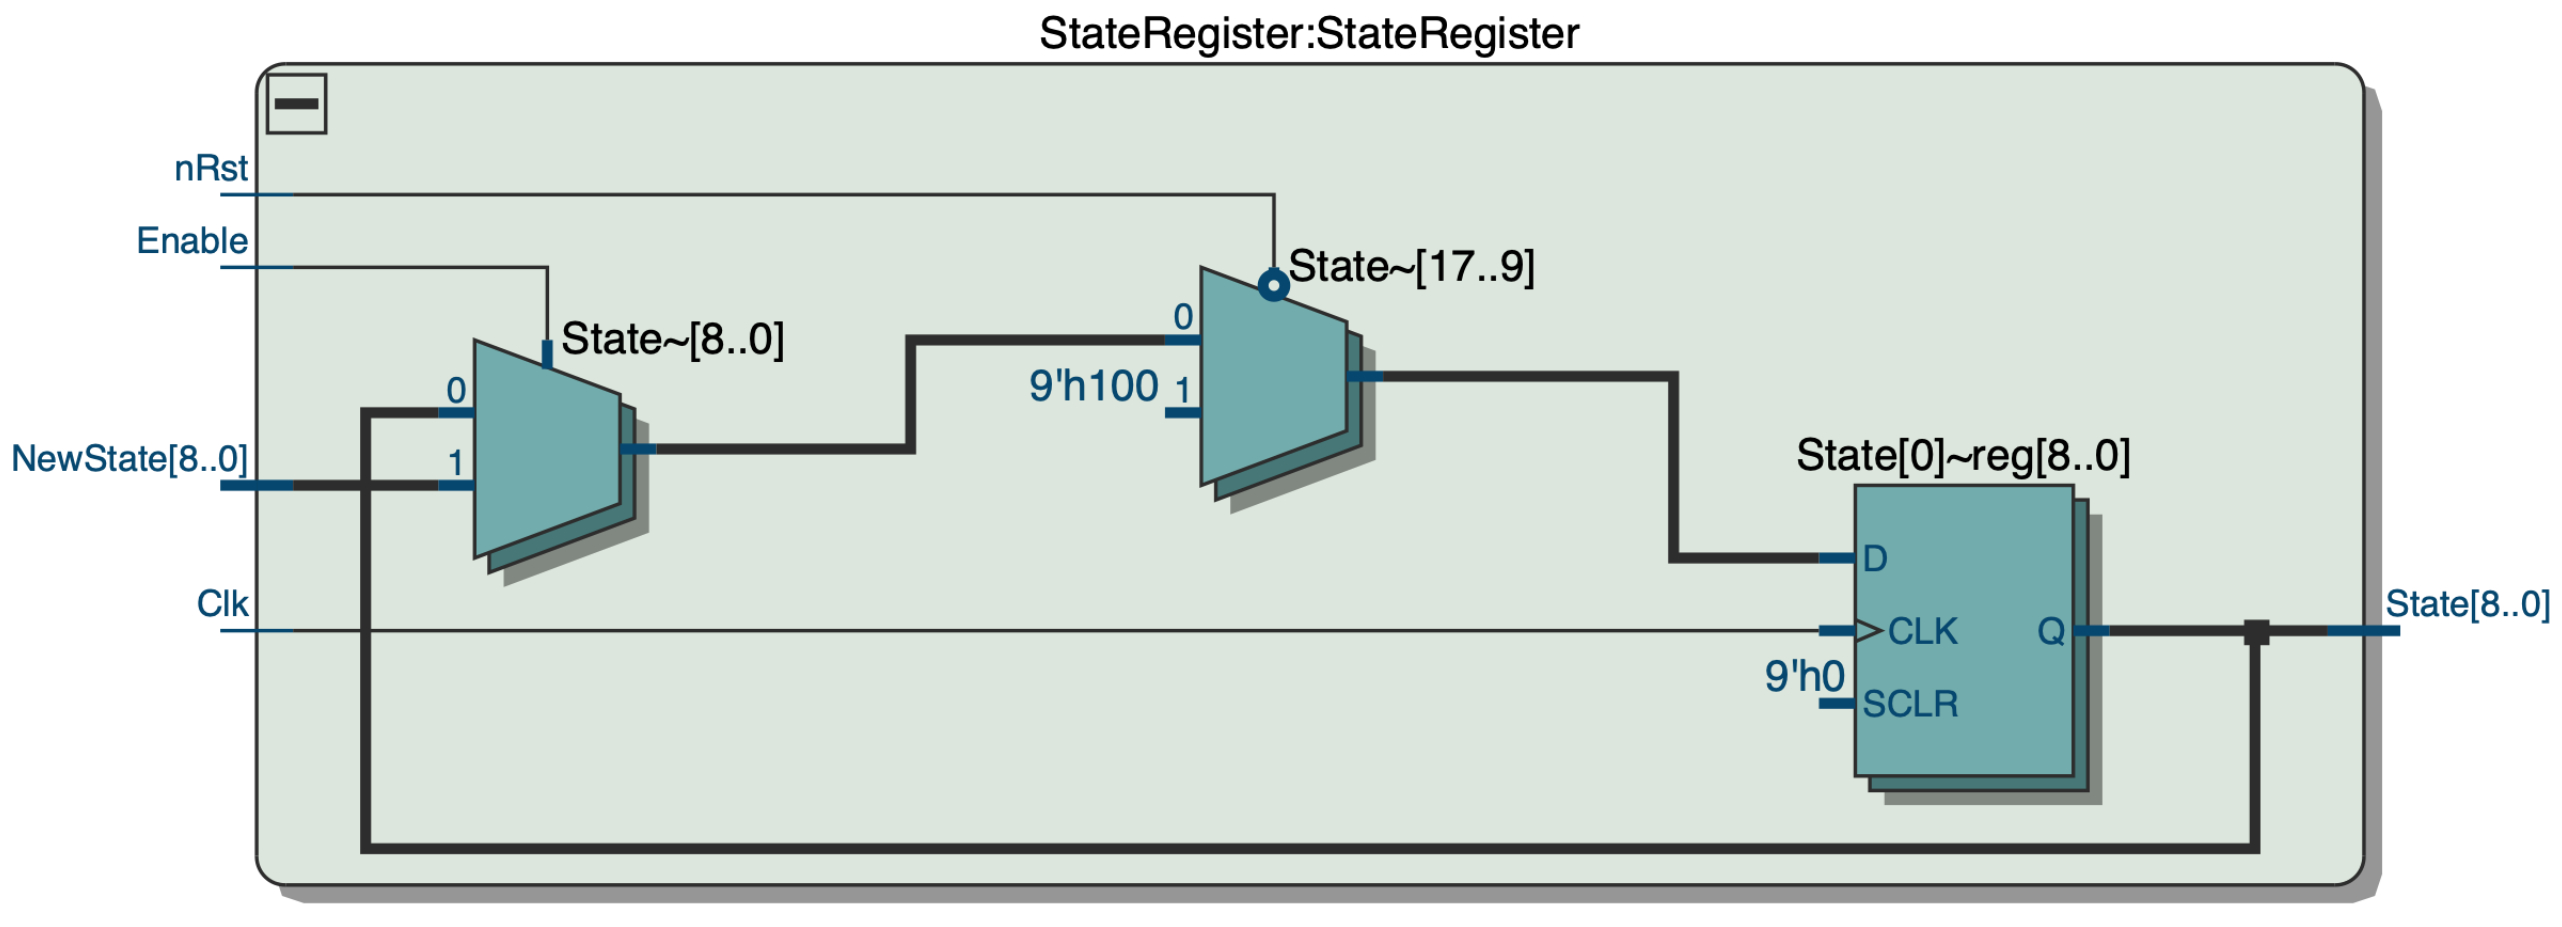
\includegraphics[width=1\textwidth]{Figures/Part1_RTL_StateRegister_old.jpg}
    \figcaption{RTL of the State register with non zero reset}
    \label{fig:p1_RTL_StateReg_old}
\end{figure}

\clearpage
\begin{figure}[h]
    \centering
    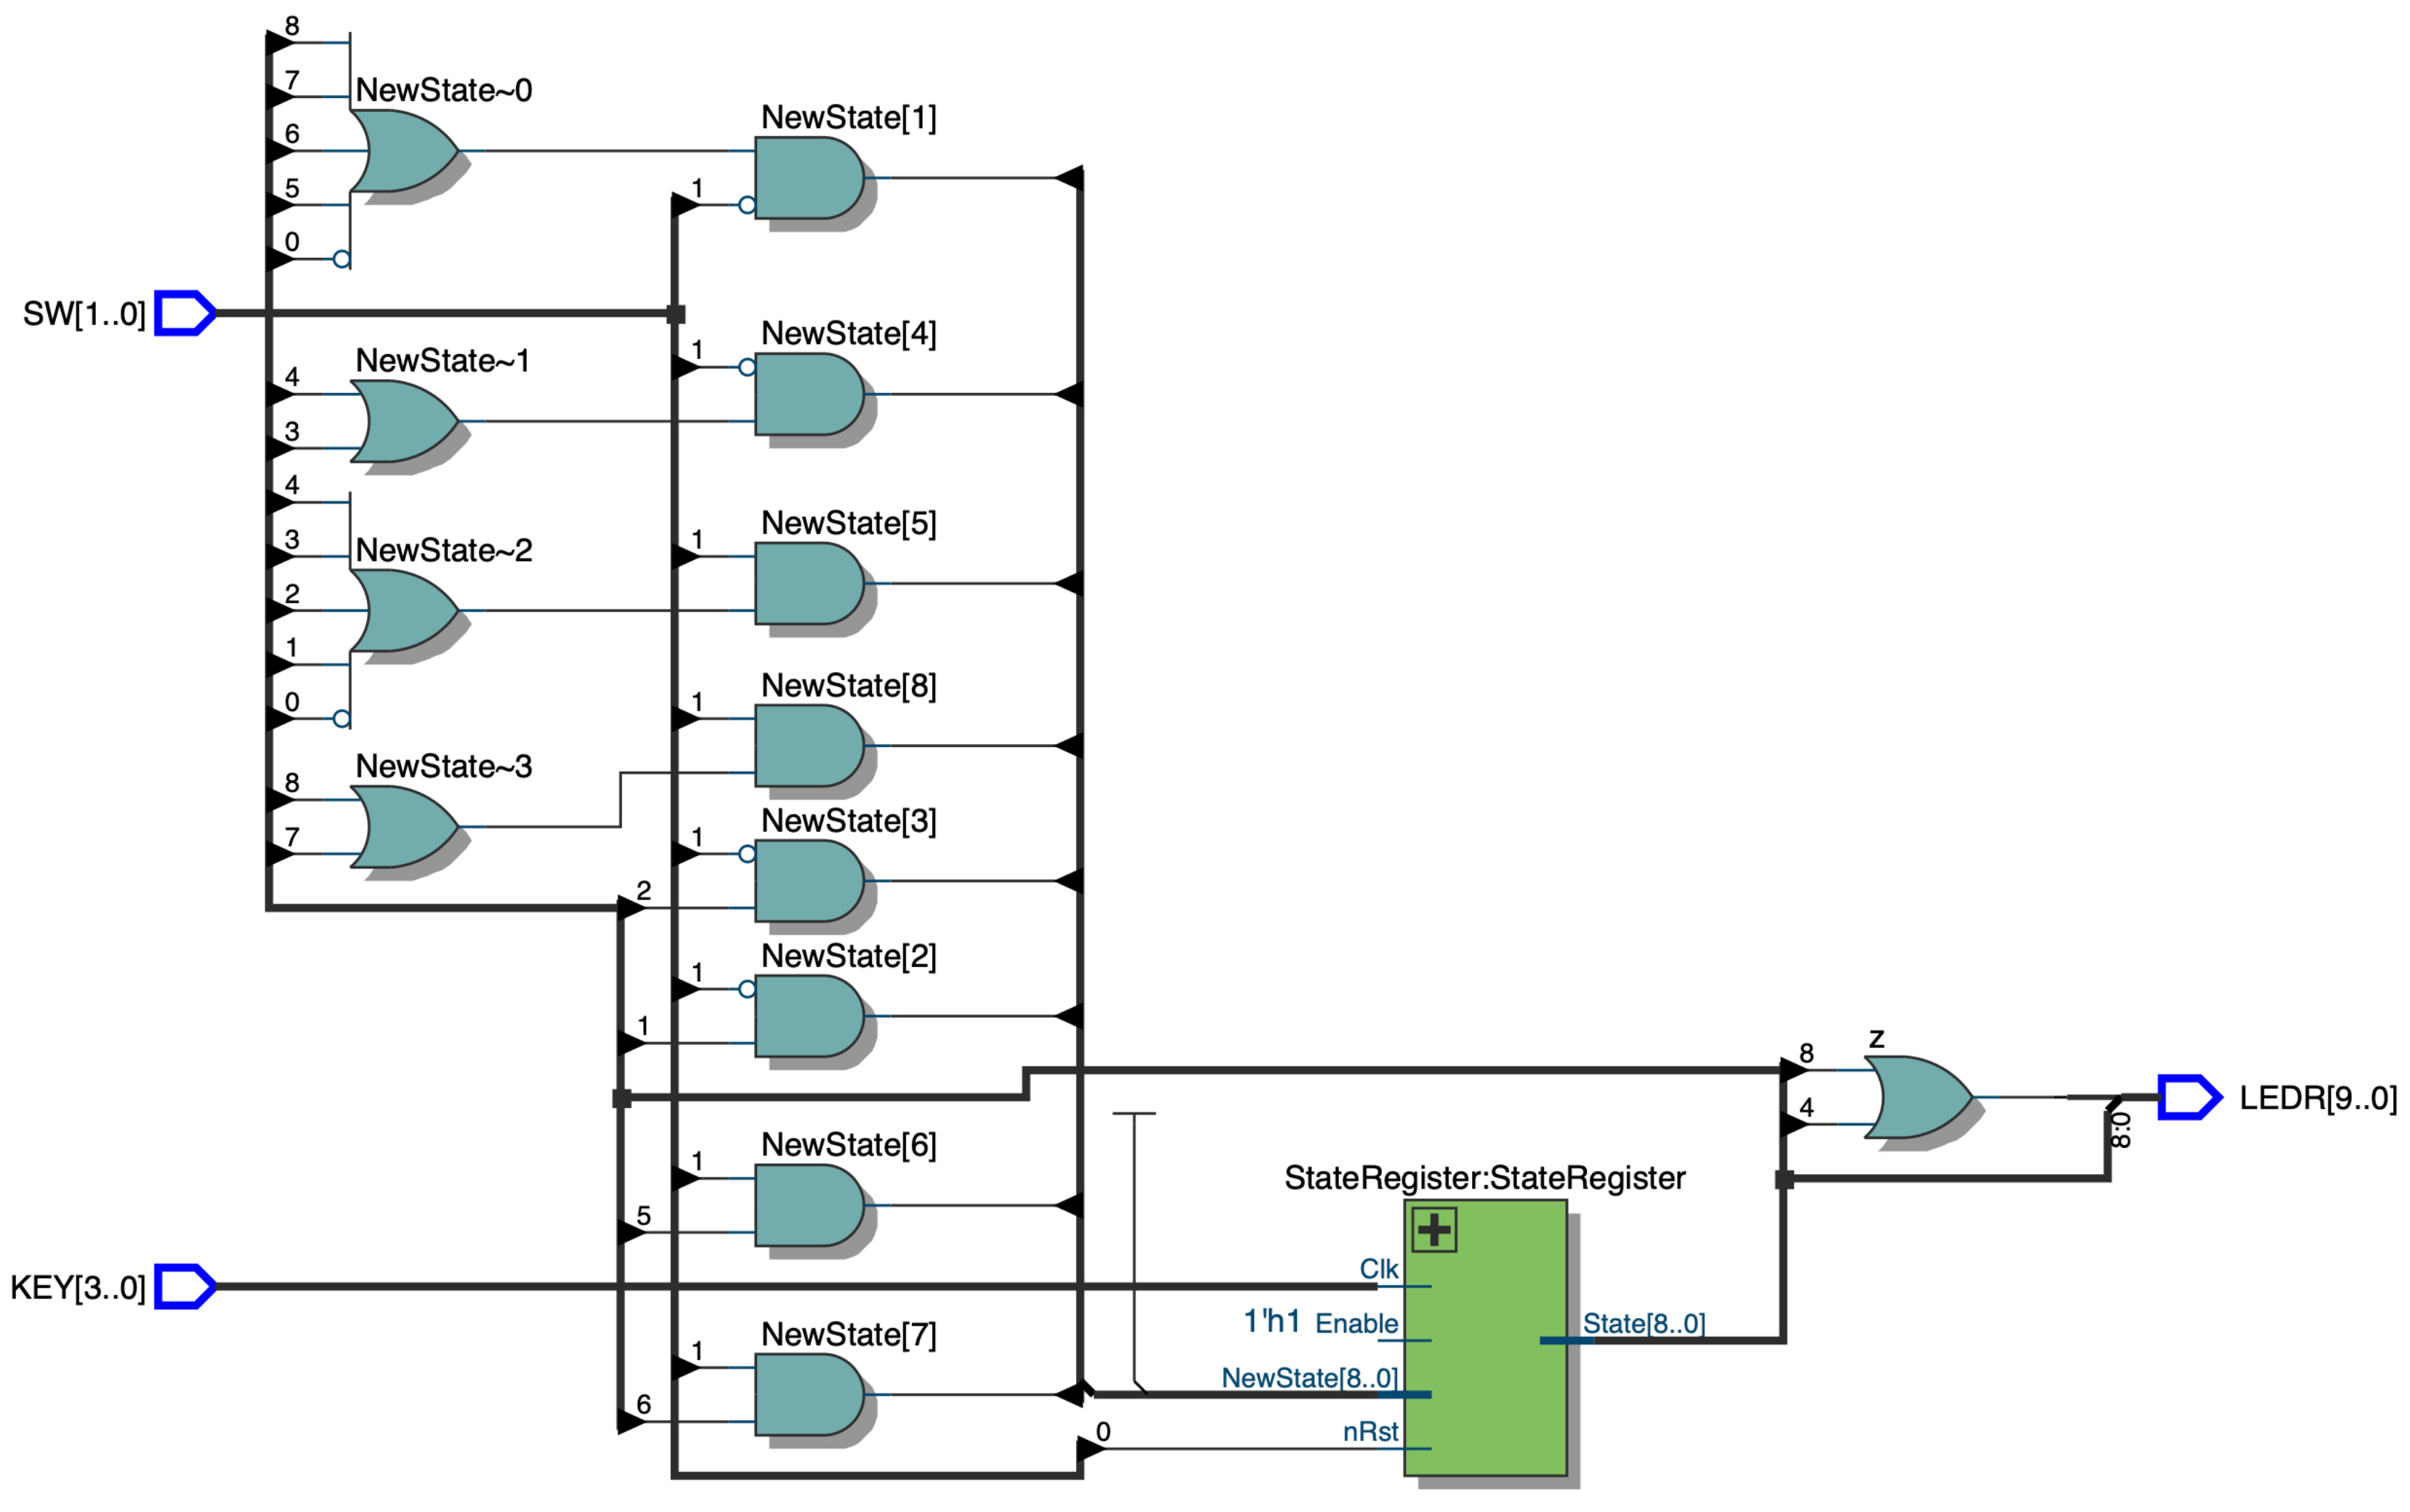
\includegraphics[width=1\textwidth]{Figures/Part1_RTL_TLE_new.jpg}
    \figcaption{RTL of the TLE with the second type one-hot encoding}
    \label{fig:p1_RTL_TLE_new}
\end{figure}
\hfill
\begin{figure}[h]
    \centering
    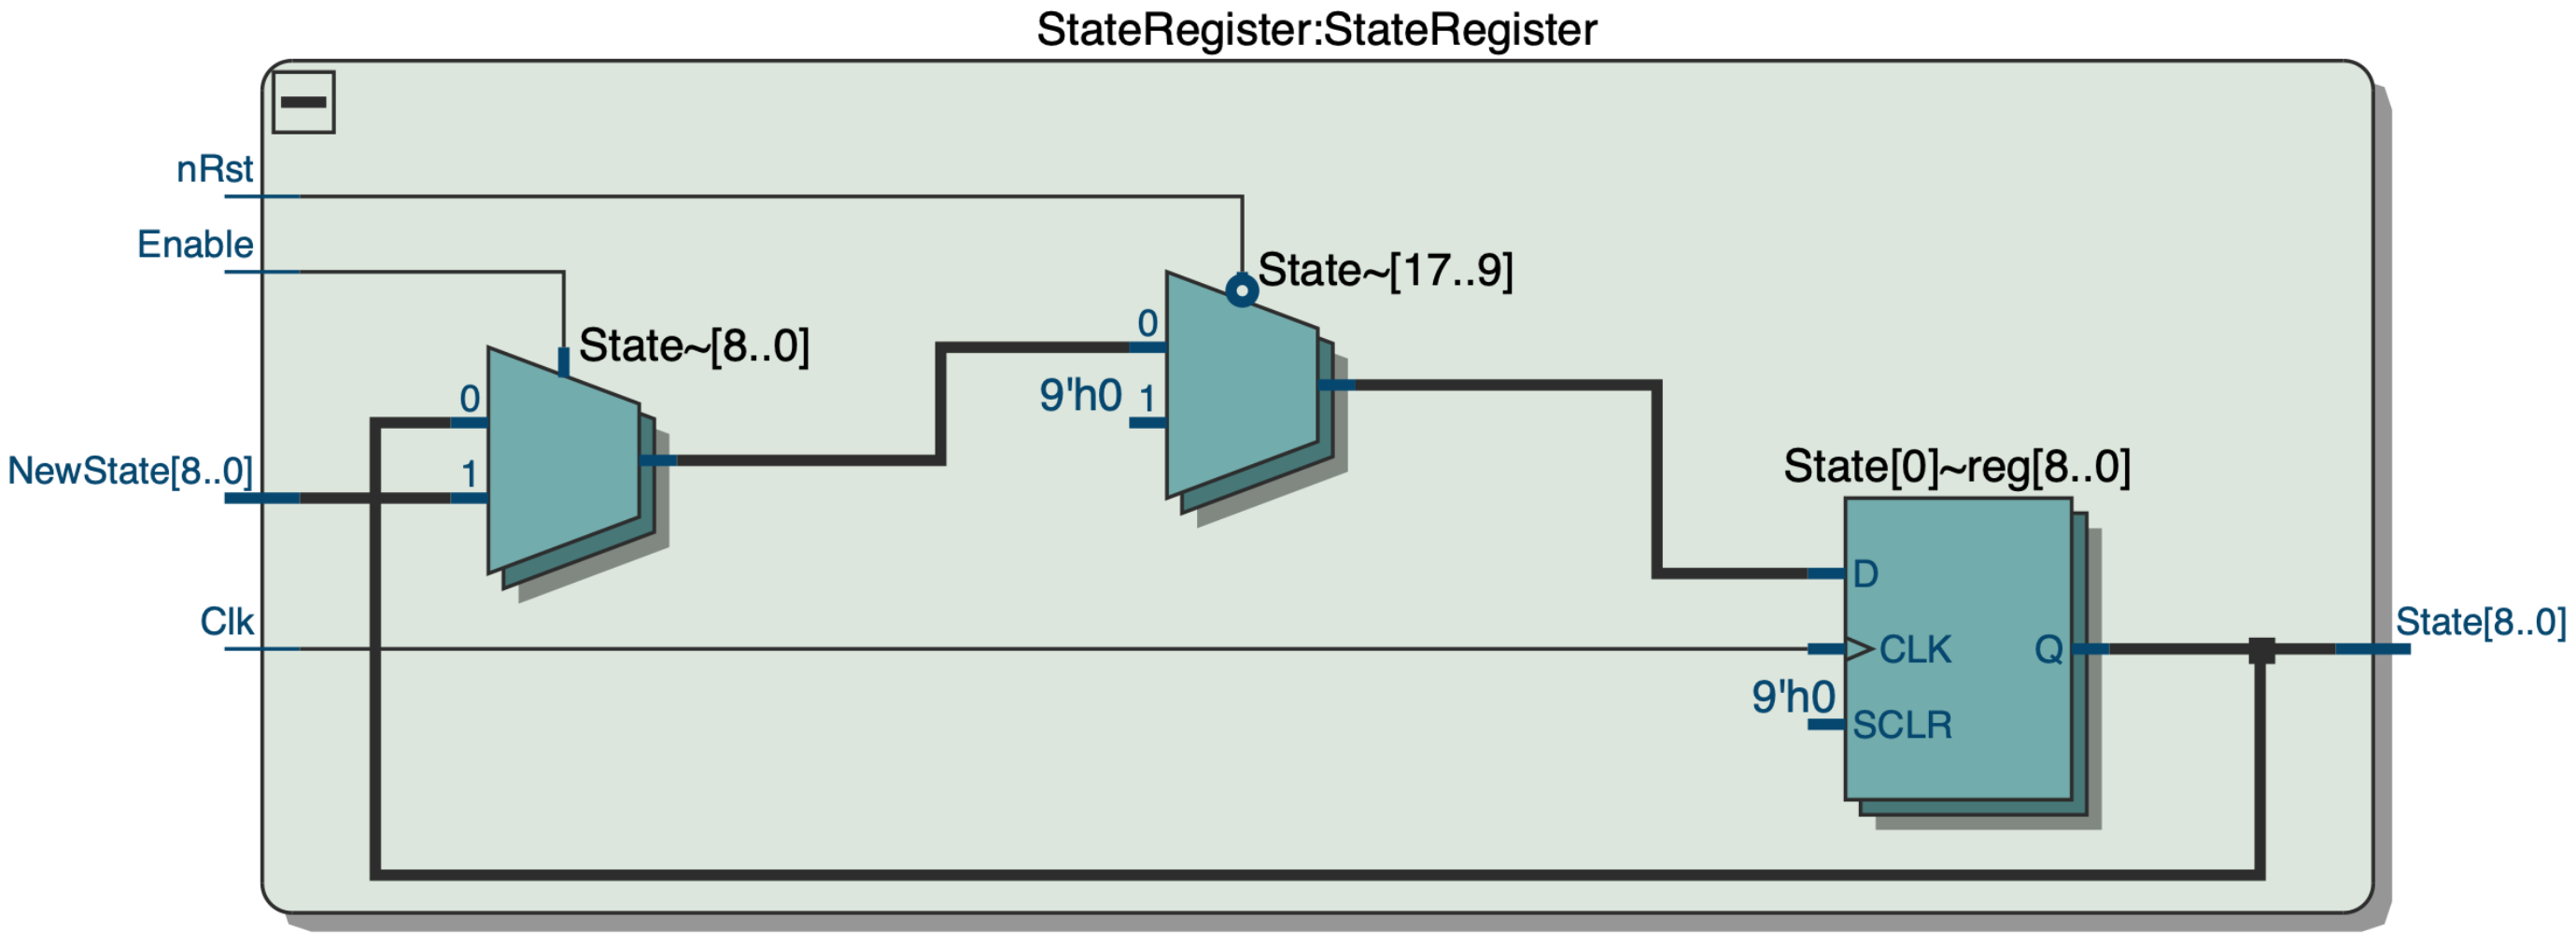
\includegraphics[width=1\textwidth]{Figures/Part1_RTL_StateRegister_new.jpg}
    \figcaption{RTL of the State register with true zero reset}
    \label{fig:p1_RTL_StateReg_new}
\end{figure}

As clearly visible there is not much difference between these two types of encoding.

\clearpage
\subsection{Results}
Showing the function of the circuit is hard with photos, therefore videos is uploaded to YouTube. Here is the video showing the \href{https://youtu.be/Wk256vCVhfY}{first encoding type} and the \href{https://youtu.be/uTf9eZYBo-c}{second encoding type}\par
In case linking is not working, the full URLs is below: \par
\url{https://youtu.be/Wk256vCVhfY}\par
\url{https://youtu.be/uTf9eZYBo-c}




%   ############################## Section ##############################
\section{Part 2}
This Part is about making a FSM using behavioural architecture, and the encoding should be binary. The complier info for the encoding could be checked and then change the encoding to one-hot and check again.

\subsection{Solving}
Solving this task was done by making a new variable type for the different states then making a State variable and setting it to the different states using a case when system. This was done three times, one case when for changing state, here a custom procedure was implemented, not necessary but increases readability. Then a case when for the output, which is only on for the two "last" states. Then a final output case when is only made for displaying the current state encoding on the first 4 LED's. \verb|type is "sequential"| forces binary encoding. This was simply replaced with \verb|type is "one-hot"| for checking compilation with this different encoding.

\subsection{Code}
\writecode[VHDL]{Part2_TLE.vhd}{TLE for the behavioural FSM}

\clearpage
\subsection{RTL}

\begin{figure}[h]
    \centering
    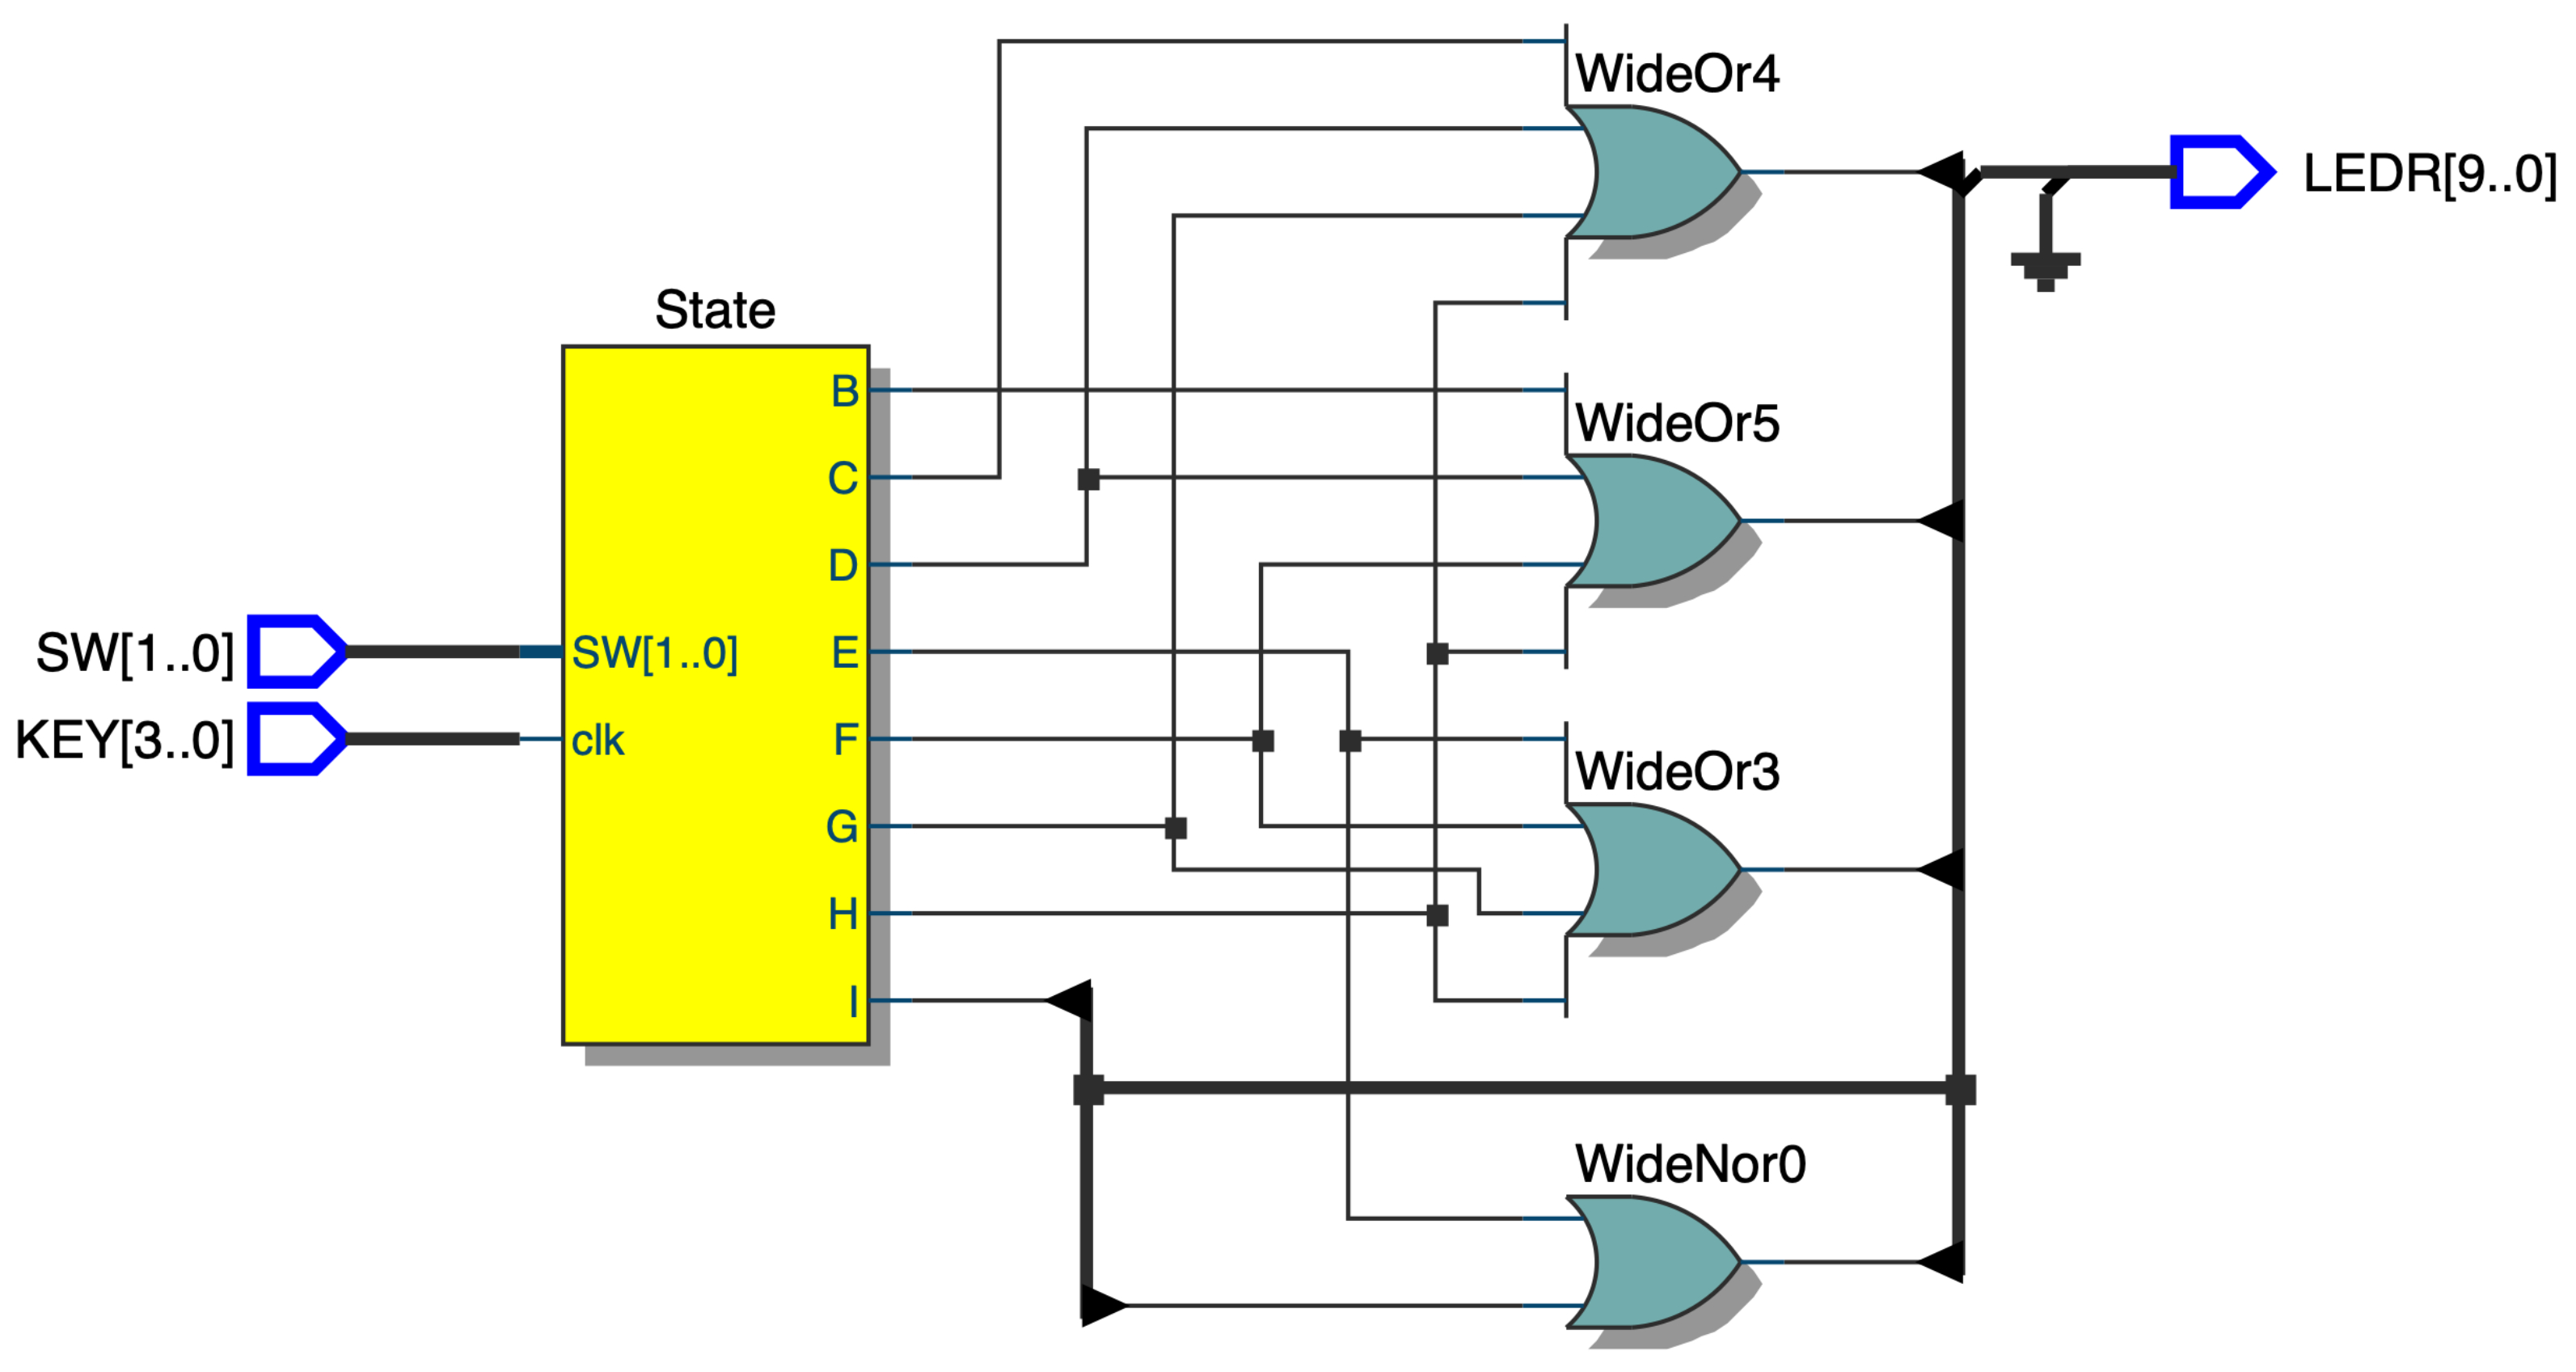
\includegraphics[width=1\textwidth]{Figures/Part2_RTL_TLE.jpg}
    \figcaption{RTL of the TLE}
    \label{fig:p2_RTL_TLE}
\end{figure}
\hfill
\begin{figure}[h]
    \centering
    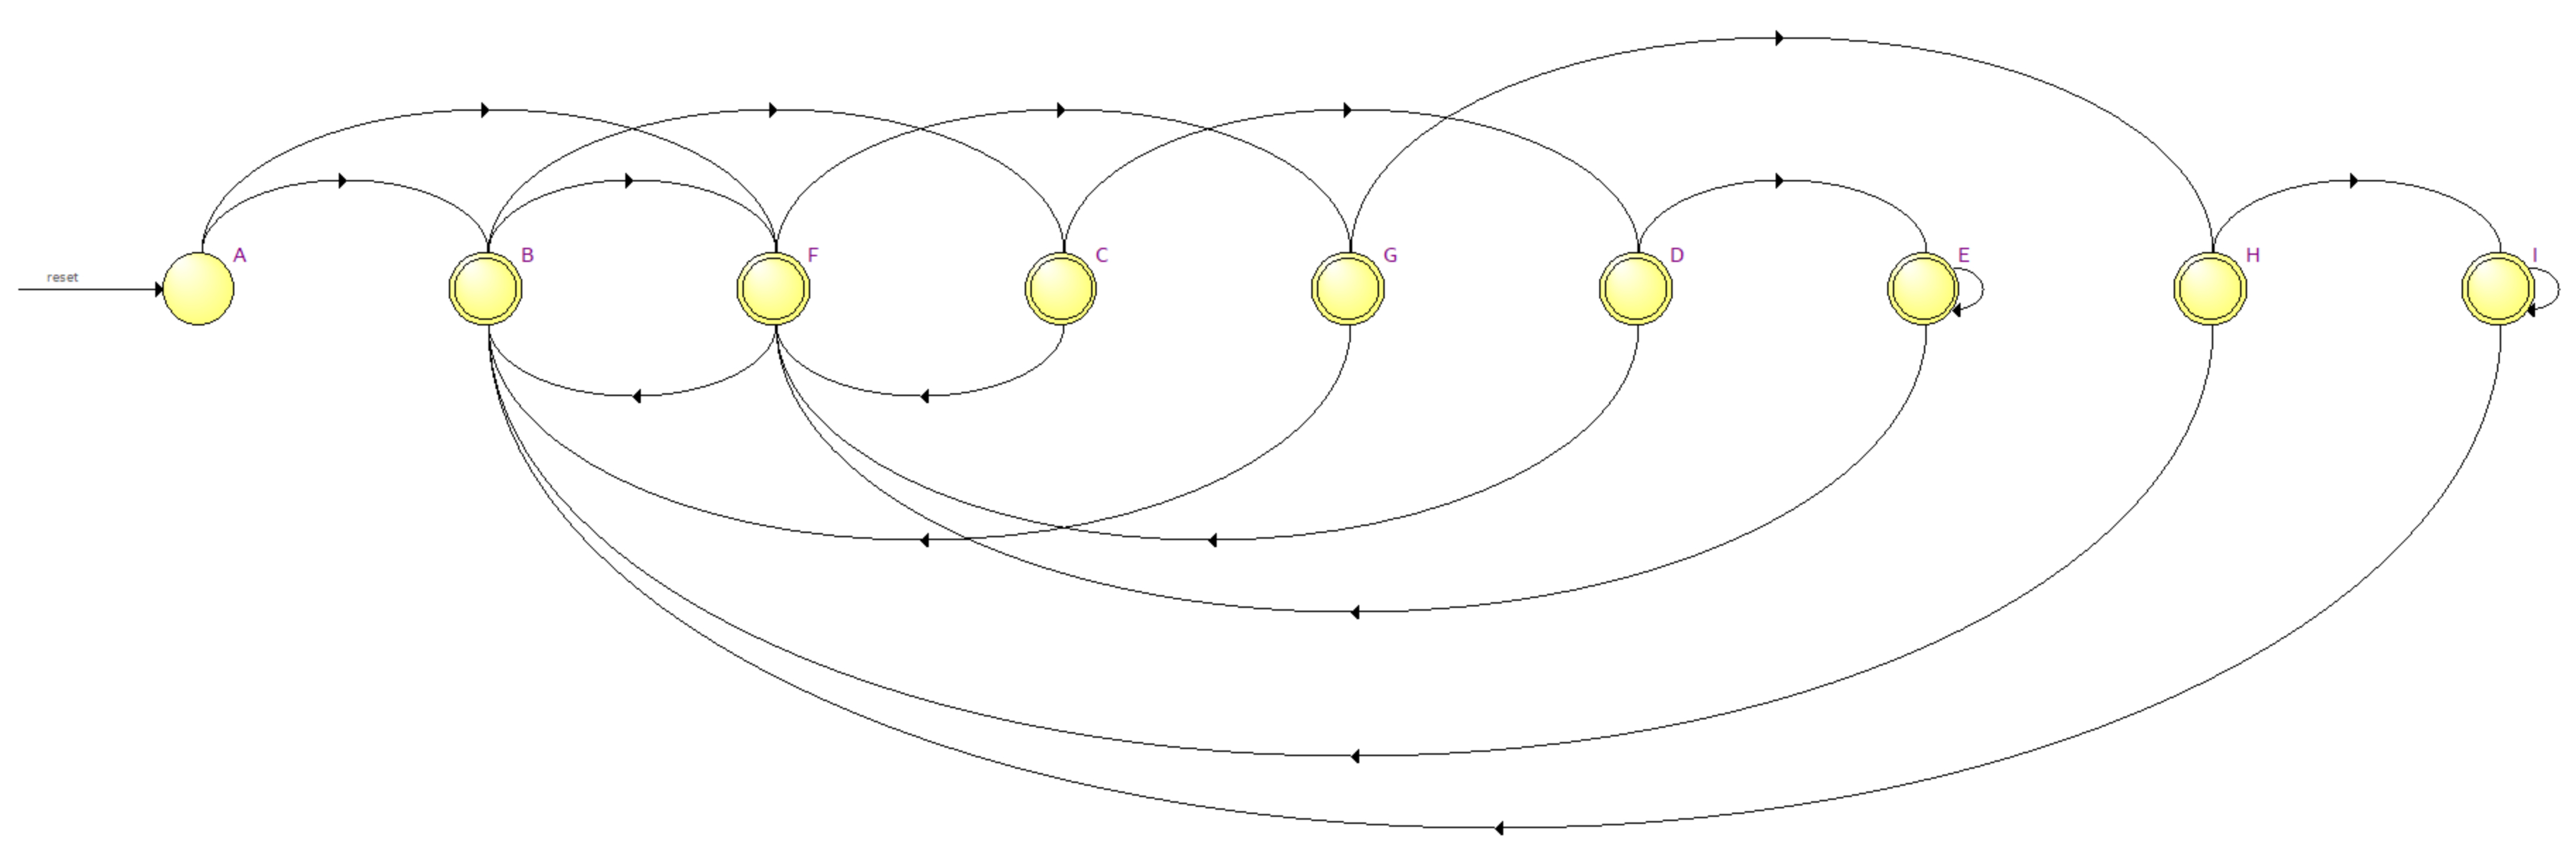
\includegraphics[width=1\textwidth]{Figures/StateSequential.jpg}
    \figcaption{State diagram}
    \label{fig:p2_states}
\end{figure}

\clearpage
Below the State diagram the used encoding shows up in a table. Instead of supplying a screenshot with bad quality, it was re-typed in excel with the same information and then imported here. The full screenshots from the FSM views is found on the \linkgithub{GitHub}

% Table generated by Excel2LaTeX from sheet 'Part 2 Output'
\begin{table}[htbp]
  \centering
  \tabcaption{Bit encoding output with sequential type}
    \begin{tabular}{|c|c|c|c|c|}
    \hline
    State & \multicolumn{4}{c|}{Encoding} \bigstrut\\
\cline{2-5}    Name  & 3     & 2     & 1     & 0 \bigstrut\\
    \hline
    A     & 0     & 0     & 0     & 0 \bigstrut\\
    \hline
    B     & 0     & 0     & 0     & 1 \bigstrut\\
    \hline
    C     & 0     & 0     & 1     & 0 \bigstrut\\
    \hline
    D     & 0     & 0     & 1     & 1 \bigstrut\\
    \hline
    E     & 0     & 1     & 0     & 0 \bigstrut\\
    \hline
    F     & 0     & 1     & 0     & 1 \bigstrut\\
    \hline
    G     & 0     & 1     & 1     & 0 \bigstrut\\
    \hline
    H     & 0     & 1     & 1     & 1 \bigstrut\\
    \hline
    I     & 1     & 0     & 0     & 0 \bigstrut\\
    \hline
    \end{tabular}%
  \label{tab:out_seq}%
\end{table}%

% Table generated by Excel2LaTeX from sheet 'Part 2 Output'
\begin{table}[htbp]
  \centering
  \tabcaption{Bit encoding output with one-hot type}
    \begin{tabular}{|c|c|c|c|c|c|c|c|c|c|}
    \hline
    State & \multicolumn{9}{c|}{Encoding} \bigstrut\\
\cline{2-10}    Name  & 8     & 7     & 6     & 5     & 4     & 3     & 2     & 1     & 0 \bigstrut\\
    \hline
    A     & 0     & 0     & 0     & 0     & 0     & 0     & 0     & 0     & 0 \bigstrut\\
    \hline
    B     & 0     & 0     & 0     & 0     & 0     & 0     & 0     & 1     & 1 \bigstrut\\
    \hline
    C     & 0     & 0     & 0     & 0     & 0     & 0     & 1     & 0     & 1 \bigstrut\\
    \hline
    D     & 0     & 0     & 0     & 0     & 0     & 1     & 0     & 0     & 1 \bigstrut\\
    \hline
    E     & 0     & 0     & 0     & 0     & 1     & 0     & 0     & 0     & 1 \bigstrut\\
    \hline
    F     & 0     & 0     & 0     & 1     & 0     & 0     & 0     & 0     & 1 \bigstrut\\
    \hline
    G     & 0     & 0     & 1     & 0     & 0     & 0     & 0     & 0     & 1 \bigstrut\\
    \hline
    H     & 0     & 1     & 0     & 0     & 0     & 0     & 0     & 0     & 1 \bigstrut\\
    \hline
    I     & 1     & 0     & 0     & 0     & 0     & 0     & 0     & 0     & 1 \bigstrut\\
    \hline
    \end{tabular}%
  \label{tab:out_oh}%
\end{table}%

\clearpage
\subsection{Results}
Showing the function of the circuit is hard with photos, therefore a video is uploaded to YouTube. Here is the video showing the \href{https://youtu.be/ZBt7R3HuPg0}{behavioural state} with the hardcoded output equal to the \verb|type is "sequential"| encoding\par
In case linking is not working, the full URL is below: \par
\url{https://youtu.be/ZBt7R3HuPg0}


\end{document}
